\graphicspath{{content/chapters/2_background/figures/}}
\chapter{Background}
\label{chp:background}

In this chapter, background information on established classical noise reduction methods is provided. These methods align with the scope of the project in that they do not require any reference or clean signal to base their predictions on. The chapter explores the Spectral Subtraction method and the Wiener Filtering method. Additionally, a brief section outlining the progression of the project and relevant foundational knowledge is included.

\section{Spectral Subtraction}
\label{sec:spectral_subtraction}

Spectral Subtraction is one of the most widely used techniques for single-channel speech enhancement. The core idea is to estimate the noise spectrum from a noisy speech signal and subtract it from the observed spectrum to obtain a cleaner signal \cite{loizou2013speech}. It assumes that noise remains relatively stationary over short time frames, while speech is a dynamic, non-stationary signal.

For digital signal processing to occur, the analog speech signal \(x(t)\), which is continuous in time, must first be converted into a digital signal \(x[n]\), a discrete-time representation. This digitisation must satisfy the Nyquist criterion: the sampling rate should be at least twice the maximum frequency component present in the signal to ensure accurate reconstruction. However, sampling inherently introduces limitations. Quantisation noise, resulting from the finite precision of digital systems, and aliasing, caused by inadequate sampling rates, can degrade the signal. If the sampling rate is too low, high-frequency components may fold into lower frequencies, misrepresenting the signal content.

\begin{figure}[h]
    \centering
    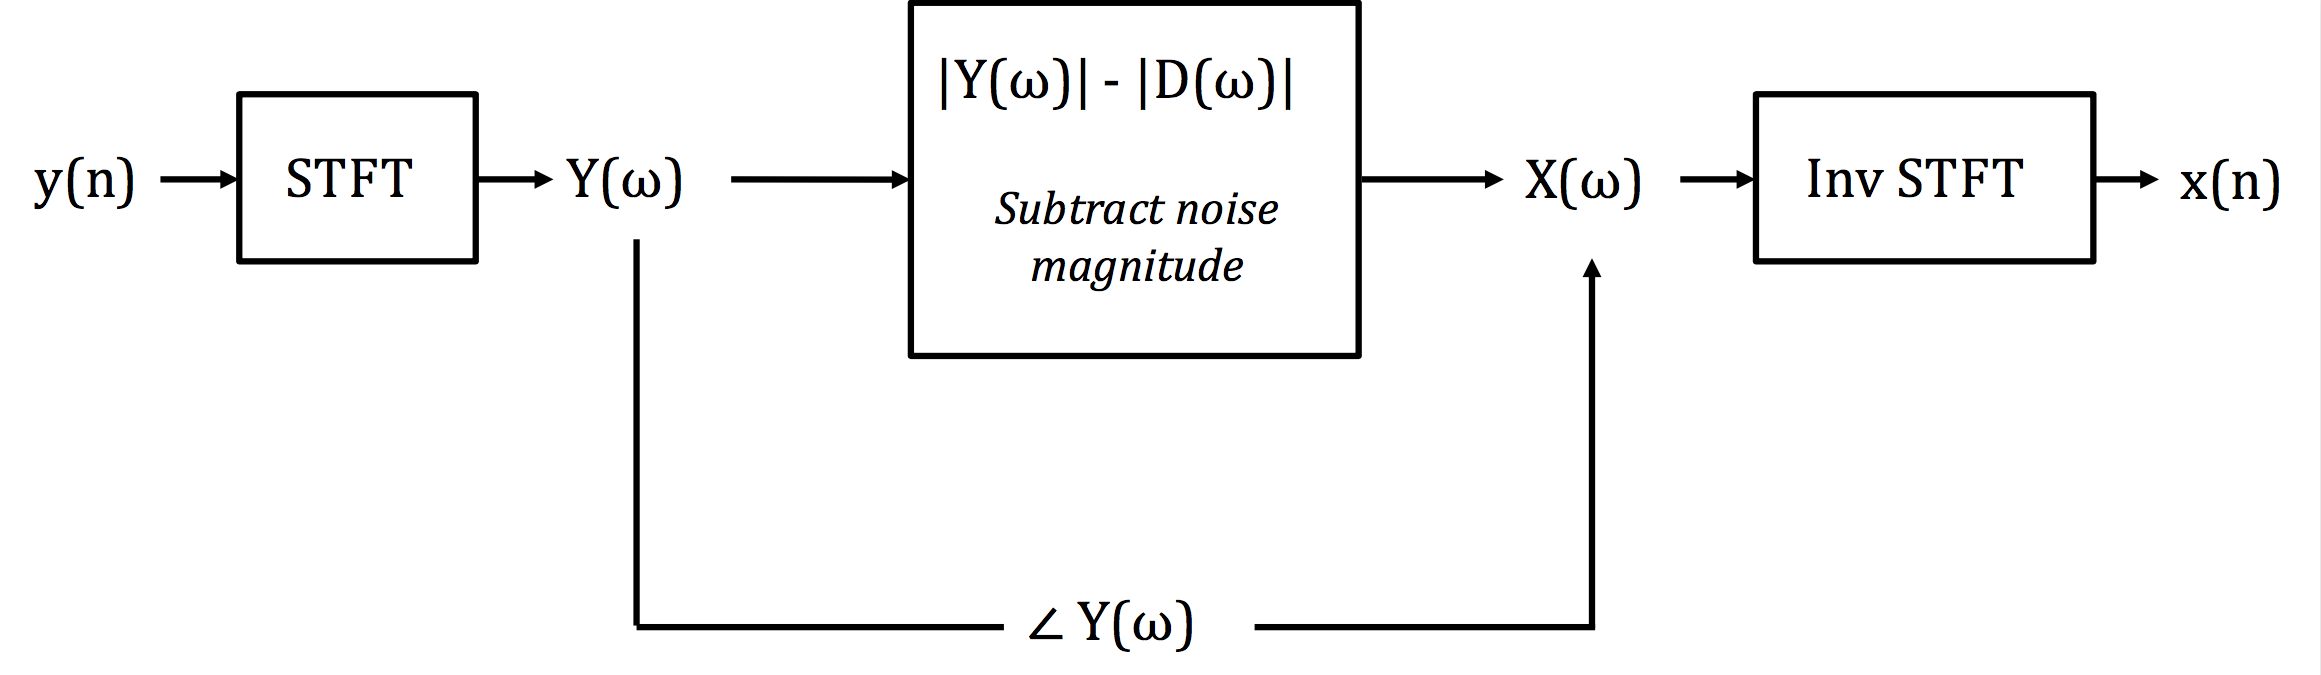
\includegraphics[width=\textwidth,keepaspectratio]{specsub.png}
    \caption{\label{fig:SSBlock} Block diagram of the Spectral Subtraction method \cite{dubey2016evaluation}.}
\end{figure}

Before applying spectral subtraction, the signal is pre-processed into a suitable format using the Short-Time Fourier Transform (STFT). The STFT segments the time-domain signal into overlapping frames using a windowing function and then converts each segment into the frequency domain. Windowing reduces spectral leakage and preserves continuity in the frequency domain. The magnitude spectrum of the noisy signal is obtained by taking the absolute value of the STFT \cite{dubey2016evaluation}. The noise spectrum is estimated by averaging the spectral magnitudes of non-speech segments over time. Once this estimate is obtained, it is subtracted from the noisy spectrum to yield an estimate of the clean speech. The final step applies the Inverse Short-Time Fourier Transform (ISTFT) to reconstruct the enhanced signal in the time domain by summing the overlapping frames.

This process can be mathematically described as:

\begin{equation}
    |X(\omega)| = |Y(\omega)| - |D(\omega)|
\end{equation}

where:
\begin{itemize}
    \item \( X(\omega) \): Estimated clean speech spectrum,
    \item \( Y(\omega) \): Magnitude spectrum of the noisy speech,
    \item \( D(\omega) \): Estimated noise spectrum.
\end{itemize}

Spectral subtraction is widely adopted due to its simplicity and low computational cost. It requires only a single input channel and is straightforward to implement. However, it comes with notable limitations. It assumes stationary noise—a condition often unmet in real environments—and may introduce **musical noise**, a type of distortion perceived as tonal artifacts. Additionally, excessive subtraction may distort speech, while insufficient subtraction can leave residual noise.

Despite these challenges, spectral subtraction remains a valuable baseline for evaluating more advanced noise suppression techniques. Methods such as Wiener filtering and deep learning-based approaches have been developed to overcome these shortcomings through more adaptive or data-driven mechanisms \cite{loizou2013speech}.


\section{Wiener Filtering}
\label{sec:wiener_filtering}

Wiener filtering is a statistically grounded method for speech enhancement that aims to minimise the mean square error (MSE) between the estimated clean signal and the true clean signal \cite{loizou2013speech}. Originally developed for linear time-invariant systems, the Wiener filter assumes that both the signal and noise are stationary stochastic processes and seeks the optimal linear estimate of the clean speech given the noisy observation \cite{dubey2016evaluation}.

The method can be applied in both the time domain and frequency domain, though the frequency domain approach is more common in speech processing due to its computational efficiency and alignment with standard short-time signal representations. The key idea is that if the power spectral densities (PSDs) of the clean speech \(P_S(\omega)\) and the noise \(P_N(\omega)\) are known or can be estimated, the optimal filter \(H(\omega)\) is derived as:

\begin{equation}
    H(\omega) = \frac{P_S(\omega)}{P_S(\omega) + P_N(\omega)}
\end{equation}

This filter acts as a frequency-dependent gain function. Frequencies where the clean speech dominates (\(P_S \gg P_N\)) are preserved, while noise-dominant frequencies (\(P_N \gg P_S\)) are attenuated. The enhanced speech spectrum is obtained by multiplying the noisy spectrum \(Y(\omega)\) with the Wiener gain:

\begin{equation}
    \hat{X}(\omega) = H(\omega)Y(\omega)
\end{equation}

Following this, the enhanced time-domain signal is reconstructed using the Inverse Short-Time Fourier Transform (ISTFT).

\begin{figure}[h]
    \centering
    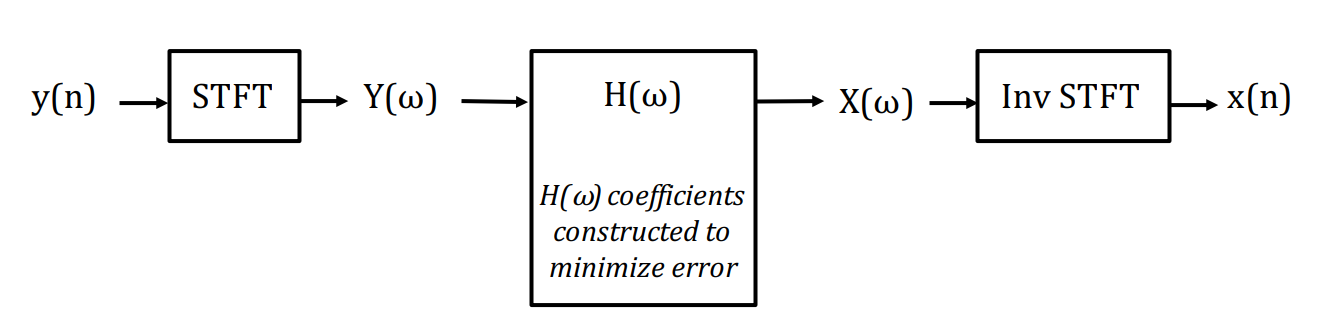
\includegraphics[width=0.95\textwidth,keepaspectratio]{wiener_block.png}
    \caption{\label{fig:WienerBlock} Block diagram of the Wiener filtering process \cite{dubey2016evaluation}.}
\end{figure}

In the time domain, the Wiener filter can be derived through a least mean square (LMS) optimisation approach. Consider a noisy signal \( y(n) = x(n) + d(n) \), where \( x(n) \) is the clean signal and \( d(n) \) is the noise. The filter \( h(n) \) is constructed to minimise the expected squared error:

\begin{equation}
    J = E\left[ (x(n) - \hat{x}(n))^2 \right]
\end{equation}

Expanding this using the LMS framework, the optimal filter is:

\begin{equation}
    h = R_{yy}^{-1} r_{yx}
\end{equation}

where \( R_{yy} \) is the autocorrelation matrix of the noisy signal and \( r_{yx} \) is the cross-correlation vector between the noisy and clean signals. The result is then convolved with \( y(n) \) to obtain the enhanced estimate \( \hat{x}(n) \).

Wiener filtering is particularly advantageous when the noise characteristics can be reliably estimated, such as during silent segments of speech. However, it assumes that the noise is zero-mean and uncorrelated with the speech signal, which may not always hold in practice. Additionally, in highly non-stationary environments, its performance can degrade due to inaccurate PSD estimates.Compared to spectral subtraction, Wiener filtering provides a more principled and statistically optimal approach, balancing noise suppression and speech preservation based on spectral power estimates. It introduces less musical noise and generally achieves better perceptual quality in stationary noise conditions.

Wiener filtering can be seen toprovide an optimal solution in the minimum mean square error (MMSE) sense. It is able to retain the spectral shape of speech components better than spectral subtraction, making it a more effective method for speech enhancement. The Wiener filter is adaptable to both time and frequency domain implementations, allowing for flexibility in its application. However, it assumses stationary noise and accurate noise estimation, which may not always hold in real-world scenarios. This can lead to over-smoothing, reducing speech intelligibility. Additionally, the performance of Wiener filtering can degrade in highly dynamic or non-stationary noise conditions.

Despite its assumptions, Wiener filtering is still widely used as a foundational method in speech enhancement and often forms part of more complex hybrid pipelines or adaptive filtering systems \cite{dubey2016evaluation, loizou2013speech}.


\section{Evaluation Metrics}
\label{sec:evaluation_metrics}

To evaluate the performance of noise reduction algorithms, several objective metrics are commonly used. These metrics provide quantitative measures of the quality and intelligibility of enhanced speech signals when compared to their clean references. The following subsections describe the most widely adopted metrics in speech enhancement research, all of which are utilised in this project.

\subsection{Signal-to-Noise Ratio (SNR)}
\label{subsec:snr}

The Signal-to-Noise Ratio (SNR) is a fundamental metric that quantifies the relative strength of the desired speech signal compared to the background noise. A higher SNR indicates better separation between speech and noise components, which typically translates to improved intelligibility and perceived quality.

SNR is defined as:

\begin{equation}
    \text{SNR} = 10 \log_{10} \left( \frac{P_s}{P_n} \right)
\end{equation}

where \( P_s \) is the power of the clean speech signal and \( P_n \) is the power of the noise (or error) component. In practice, SNR can be computed in both time and frequency domains and is commonly used as a baseline performance indicator for denoising systems.

\subsection{Mean Squared Error (MSE)}
\label{subsec:mse}

The Mean Squared Error (MSE) measures the average squared difference between the enhanced and reference clean signals. It reflects the overall fidelity of the enhancement process but does not necessarily correlate with perceptual quality.

MSE is given by:

\begin{equation}
    \text{MSE} = \frac{1}{N} \sum_{n=1}^{N} (x(n) - \hat{x}(n))^2
\end{equation}

where \( N \) is the number of signal samples, \( x(n) \) is the clean signal, and \( \hat{x}(n) \) is the enhanced signal. Lower MSE values indicate better approximation of the clean signal.

\subsection{Perceptual Evaluation of Speech Quality (PESQ)}
\label{subsec:pesq}

The Perceptual Evaluation of Speech Quality (PESQ) is an objective metric designed to estimate the perceptual quality of speech, taking into account human auditory perception. Standardised by ITU-T Recommendation P.862, PESQ is widely used in speech enhancement and telecommunication systems.

PESQ simulates the auditory perception process and compares the clean and enhanced signals using psychoacoustic models. The PESQ score ranges from -0.5 to 4.5, with higher scores indicating better perceptual quality. A score above 3.0 is generally considered acceptable for most applications.

\subsection{Short-Time Objective Intelligibility (STOI)}
\label{subsec:stoi}

The Short-Time Objective Intelligibility (STOI) metric is designed to assess the intelligibility of speech, especially in noisy or distorted conditions. It works by comparing the short-time spectral envelopes of clean and enhanced speech segments.

The STOI score lies between 0 and 1, where higher values indicate better intelligibility. Scores above 0.5 typically suggest acceptable levels of speech understanding. STOI is particularly useful when intelligibility, rather than perceptual quality alone, is of primary concern.

\subsection{Log Spectral Distance (LSD)}
\label{subsec:lsd}

The Log Spectral Distance (LSD) metric quantifies the spectral distortion introduced by a denoising algorithm. It measures the average distance between the logarithmic power spectra of the clean and enhanced signals across time and frequency.

LSD is defined as:

\begin{equation}
    \text{LSD} = \frac{1}{F} \sum_{f=1}^{F} \sqrt{ \frac{1}{T} \sum_{t=1}^{T} \left( \log S(f, t) - \log \hat{S}(f, t) \right)^2 }
\end{equation}

where \( S(f, t) \) and \( \hat{S}(f, t) \) are the clean and enhanced magnitude spectra at frequency bin \( f \) and time frame \( t \), respectively. Lower LSD values indicate better preservation of spectral characteristics and less distortion.

\vspace{1em}
Individually, these metrics suffer to provide complete meaningful evaluations of the performance of noise reduction algorithms. For example, SNR and MSE are sensitive to the absolute power levels of the signals, while PESQ and STOI focus on perceptual aspects. Therefore, a comprehensive evaluation should consider multiple metrics to capture different dimensions of performance and together a well-rounded assessment can be achieved.


\section{Project Progression}
\label{sec:project_progression}

The initial objective of this project was to enhance speech signals corrupted by noise using traditional digital signal processing (DSP) techniques. The original scope involved implementing classical noise reduction methods, such as Spectral Subtraction and Wiener Filtering, with the intention of deploying them on an MSP432 microcontroller. These techniques were selected due to their low computational complexity and suitability for resource-constrained embedded systems.

However, early experimentation and prototyping conducted in Python revealed the inherent limitations of classical DSP methods—particularly their poor performance in non-stationary noise environments and lack of adaptability to diverse real-world conditions. While methods like Spectral Subtraction offer simplicity and efficiency, they tend to introduce musical noise artifacts and degrade intelligibility under dynamic noise conditions. Similarly, Wiener Filtering, though more mathematically rigorous, still relies on assumptions about the noise characteristics that may not hold in practical use cases.

Concurrently, the rising prominence of data-driven methods in the field of speech enhancement provided a compelling alternative. Established real-time systems such as \textit{Krisp}, \textit{NVIDIA RTX Voice}, and \textit{RNNoise} have demonstrated the effectiveness of machine learning-based models for robust noise suppression. These models, trained on large-scale paired datasets of clean and noisy speech, are capable of learning complex nonlinear mappings and generalising across a wide range of noise profiles.

Given these advancements, it became increasingly evident that machine learning offered significant advantages over classical methods. Consequently, the project scope evolved from solely implementing classical techniques on a low-power embedded platform to exploring the feasibility of deploying a lightweight machine learning-based speech enhancement model on a more capable microcontroller or embedded processor.

This shift allowed the project to align with modern trends in speech processing while retaining a practical, real-time deployment focus. It also opened opportunities to evaluate the trade-offs between classical and data-driven methods—not only in terms of performance but also in memory usage, computational cost, and real-world applicability.

Thus, the revised goal of the project became twofold: to benchmark machine learning-based noise suppression models against classical DSP methods across relevant objective metrics, and to assess the practicality of deploying such models on embedded hardware for real-time speech enhancement applications. Ultimately having project title revised from \textit{DSP Based Noise Cancellation System} to \textit{Machine Learning Noise Cancellation System} to reflect the new focus on machine learning techniques.
